\documentclass[tikz,border=3pt]{standalone}
\usepackage[utf8]{inputenc}
\usepackage[T1]{fontenc}
\usepackage{lmodern}
\renewcommand{\familydefault}{\sfdefault}
\usepackage{sansmath}\sansmath
\usepackage[american]{circuitikz}
\usepackage{pgfplots}\pgfplotsset{compat=1.18,/pgf/number format/use comma,/pgf/number format/1000 sep={.}}
\usetikzlibrary{arrows.meta,calc,positioning,decorations.pathmorphing,patterns}
% paleta del sitio
\definecolor{nar}{HTML}{E8680C}\definecolor{narc}{HTML}{FFB35C}\definecolor{hielo}{HTML}{FFF3E8}
\definecolor{tinta}{HTML}{1D1D1F}\definecolor{gris}{HTML}{6E6E73}\definecolor{lila}{HTML}{7C5CF0}
\definecolor{azul}{HTML}{2F6FD6}\definecolor{menta}{HTML}{17A673}\definecolor{coral}{HTML}{E8342A}
\ctikzset{bipoles/thickness=1.6}
\begin{document}
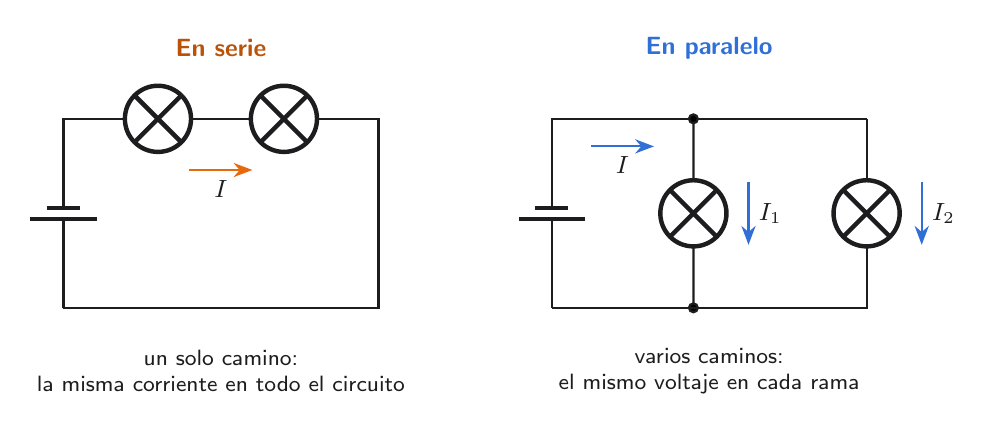
\begin{tikzpicture}[font=\small,>={Stealth[length=2.4mm]}]
\begin{scope}
\draw[tinta,thick] (0,0) to[battery1] (0,2.4) -- (0.4,2.4) to[lamp] (2,2.4) to[lamp] (3.6,2.4) -- (4,2.4) -- (4,0) -- (0,0);
\node[font=\small\bfseries,text=nar!80!black] at (2,3.3) {En serie};
\node[font=\footnotesize,align=center,text=tinta] at (2,-0.8) {un solo camino:\\la misma corriente en todo el circuito};
\draw[->,nar,thick] (1.6,1.75) -- (2.4,1.75) node[midway,below,text=tinta] {$I$};
\end{scope}
\begin{scope}[xshift=6.2cm]
\draw[tinta,thick] (0,0) to[battery1] (0,2.4) -- (4,2.4);
\draw[tinta,thick] (1.8,2.4) to[lamp,*-*] (1.8,0);
\draw[tinta,thick] (4,2.4) to[lamp] (4,0) -- (0,0);
\node[font=\small\bfseries,text=azul] at (2,3.3) {En paralelo};
\node[font=\footnotesize,align=center,text=tinta] at (2,-0.8) {varios caminos:\\el mismo voltaje en cada rama};
\draw[->,azul,thick] (0.5,2.05) -- (1.3,2.05) node[midway,below,text=tinta] {$I$};
\draw[->,azul,thick] (2.5,1.6) -- (2.5,0.8) node[midway,right,text=tinta] {$I_1$};
\draw[->,azul,thick] (4.7,1.6) -- (4.7,0.8) node[midway,right,text=tinta] {$I_2$};
\end{scope}
\end{tikzpicture}
\end{document}
